\section{Shaders}
\label{shaders}

Los shaders son programas diseñados para ejecutarse en la tarjeta gráfica\footfullcite{ogl_superbible}. A pesar de estar muy limitados, tienen la ventaja de aprovechar muy bien la capacidad de procesado paralelo de la GPU. Hoy en día los shaders son el núcleo alrededor del cual gira el renderizado de una aplicación 3D en tiempo real, y ocupan la mayor parte del tiempo de computación.

Aunque no se profundizará en lenguajes de shading, es importante saber que OpenGL ES utiliza el lenguaje de shading GLSL (OpenGL Shading Language)\footfullcite{khronos_glsl}. GLSL es un lenguaje basado en C que se compila en tiempo de ejecución mediante la API de OpenGL, a partir del propio código en texto plano. Vulkan en cambio utiliza el lenguaje intermedio SPIR-V (Standard Portable Intermediate Representation)\footfullcite{khronos_spir}. SPIR-V es el resultado de compilar GLSL mediante glslang\footfullcite{glslang} \footfullcite{spir_introduction}, y se provee en tiempo de ejecución a la API de Vulkan. Al haber sido procesado previamente SPIR-V carga sensiblemente más rápido en tiempo de ejecución. También es posible utilizar SPIR-V en OpenGL mediante una extensión (refiriéndonos a la API de escritorio, no su versión para sistemas embebidos)\footfullcite{opengl_spirext}.

En cada iteración, se ejecuta por cada elemento en escena la pipeline de la API gráfica. La pipeline recibe como parámetro una serie de primitivas (puntos, líneas o polígonos) y ejecuta los shaders pasándoles esa información. En OpenGL, la pipeline puede simplificarse como se ve en la figura \ref{fig:opengl_pipeline}.

\begin{figure}[H]
    \centering
    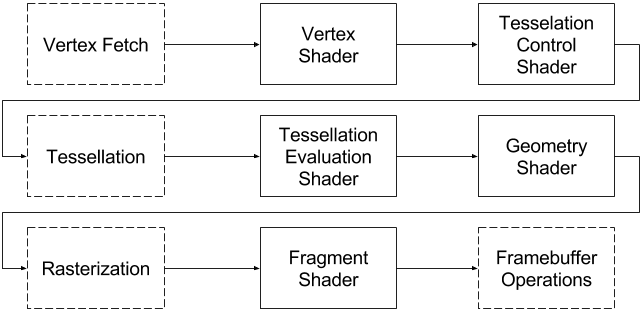
\includegraphics[width=0.80\linewidth]{ogl_pipeline}
    \caption{Esquema de la pipeline gráfica de OpenGL, adaptada directamente de OpenGL Superbible\footfullcite{ogl_superbible}.}
    \label{fig:opengl_pipeline}
\end{figure}

De esta lista, los shaders marcados con una lista discontinua no son programables, sino que tienen un comportamiento predefinido. A parte de esos, los tipos que se han utilizado para el desarrollo de la aplicación son el Vertex Shader y el Fragment Shader.

\subsection{Vertex Shader}
El Vertex Shader\footfullcite{ogl_superbible} se ejecuta independientemente por cada uno de los vértices de la malla a renderizar. Desde este shader se pueden modificar los atributos de cada uno de los vértices, recibidos desde la etapa de ``Vertex Fetch", como su posición, color, coordenadas de textura, o cualquier otra propiedad que arbitrariamente le hayamos atribuido. También pueden añadirse nuevos atributos si se desea. Una vez modificados, estos atributos se pasan como outputs del shader para ser utilizados en otros estadios de la pipeline, como el Fragment Shader.

A la hora de programar el Vertex Shader es muy importante tener en cuenta que sus datos de salida van a ser interpolados en el Fragment Shader, y también que desde un Vertex Shader no se puede acceder a los atributos de un vértice distinto al que se está procesando.

\subsection{Fragment Shader}
El Fragment Shader\footfullcite{ogl_superbible} se ejecuta por cada píxel en pantalla que ocupe cada polígono. Sus atributos de entrada son los que se han definido como salida en el Vertex Shader pero están interpolados, es decir, entre los diferentes vértices de un polígono, los píxeles de su interior tienen los atributos intermedios de cada uno de los vértices, según su proximidad a estos. También es posible enviar datos que sean únicos para todos los píxeles, como la posición de la cámara o de las luces.

Desde el Fragment Shader podemos definir el color de un píxel específico, normalmente con la ayuda de los atributos interpolados. Se utiliza especialmente para definir la cantidad y color de luz que recibe cada fragmento del polígono, en función de factores como el ángulo entre la normal de la superficie a pintar y la dirección de la luz o el ángulo respecto a la cámara.